

\documentclass{beamer}
\usetheme{default}
\usecolortheme{dove}
\usepackage{graphicx}
\usepackage{xcolor}
\usepackage{multicol}
\newcommand\independent{\protect\mathpalette{\protect\independenT}{\perp}}
\newcommand\indep{\protect\mathpalette{\protect\independenT}{\perp}}
\def\independenT#1#2{\mathrel{\rlap{$#1#2$}\mkern2mu{#1#2}}}
\definecolor{dblue}{RGB}{0,0,139}
\usepackage{tikz}
\usetikzlibrary{arrows,shapes.arrows,positioning,shapes,shapes.misc}
\usetikzlibrary{decorations.pathreplacing}
\usepackage{booktabs}
\renewcommand{\arraystretch}{1.2}
\newcommand{\Cov}{\text{Cov}}
\newcommand{\Cor}{\text{Cor}}
\newcommand{\V}{\mathbb{V}}
\renewcommand{\P}{\mathbb{P}}
\newcommand{\E}{\mathbb{E}}
\newcommand{\doop}{\text{do}}
\usepackage{hanging}% http://ctan.org/pkg/hanging
\setbeamertemplate{footnote}{%
  \hangpara{2em}{1}%
  \makebox[2em][l]{\insertfootnotemark}\footnotesize\insertfootnotetext\par%
}
\newcommand{\myfootnote}{\let\thefootnote\relax\footnote}
\newcommand{\blue}[1]{\textcolor{blue}{#1}}
\newcommand{\gray}[1]{\textcolor{gray}{#1}}
\newcommand{\green}[1]{\textcolor{olive}{#1}}
\newcommand{\purple}[1]{\textcolor{purple}{#1}}
\newcommand{\bred}[1]{\textbf{\textcolor{red}{#1}}}
\newcommand{\bblue}[1]{\textbf{\textcolor{blue}{#1}}}
\newcommand{\bgreen}[1]{\textbf{\textcolor{olive}{#1}}}
\newcommand{\bpurple}[1]{\textbf{\textcolor{purple}{#1}}}
\newcommand\black[1]{\color{black}#1}
\newcommand\white[1]{\color{white}#1}
\usepackage{array}
\newcolumntype{L}[1]{>{\raggedright\let\newline\\\arraybackslash\hspace{0pt}}m{#1}}
\usepackage[round]{natbib}
\bibliographystyle{humannat-mod}
\setbeamertemplate{footnote}{%
  \footnotesize\insertfootnotetext\par%
}
\newcommand\blfootnote[1]{%
  \begingroup
  \renewcommand\thefootnote{}\footnote{#1}%
  \addtocounter{footnote}{-1}%
  \endgroup
}
\setbeamertemplate{enumerate items}[default]
\usepackage[append]{beamersubframe}
\title{FF_slides}
\author{Ian Lundberg}
\institute[Princeton University] % (optional, but mostly needed)
{
  Department of Sociology and Office of Population Research\\
  Princeton University
}
\date{\today}

\begin{document}

\begin{frame}
\centering
\begin{tikzpicture}[x = .5\textwidth, y = .5\textheight]
\node at (-1,-1) {};
\node at (1,1) {};
\node[font={\Large\bf},blue,align=center,anchor=south] (title) at (0,.6) {Making the most of the\\Fragile Families and Child Wellbeing Study};
\node[anchor = east] at (1,0) {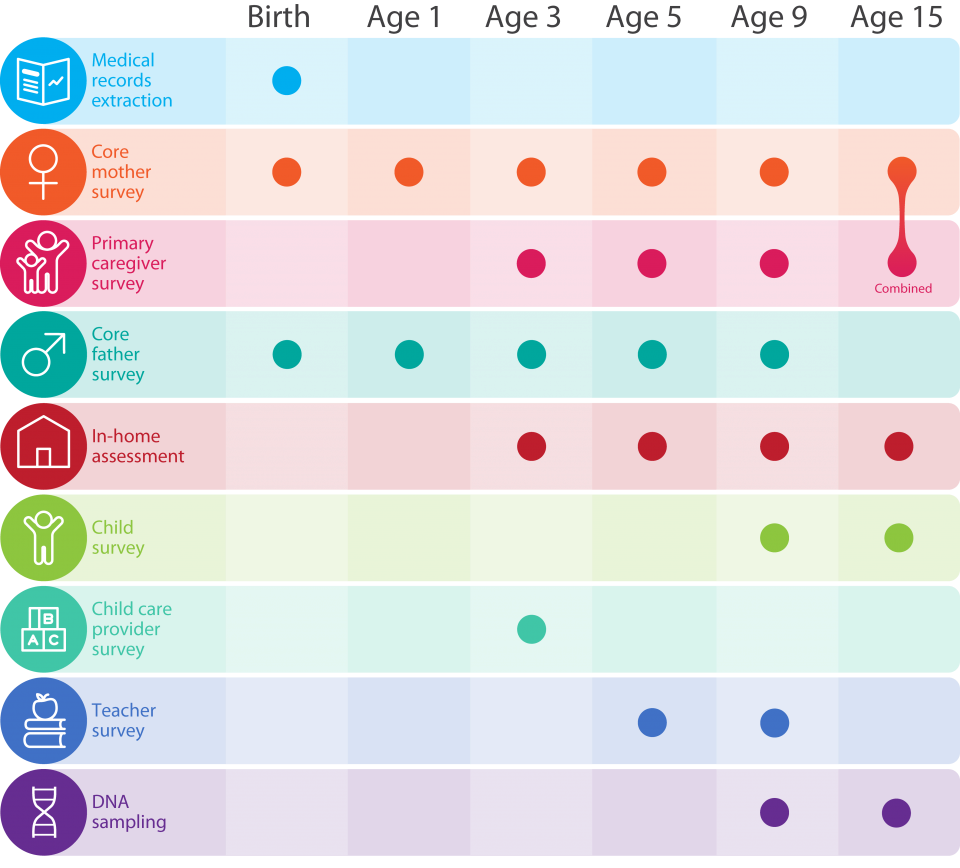
\includegraphics[width = .5\textwidth]{figures/ff_design_full}};
\node[anchor = north west,align = left] (ian) at (-1,.3) {\bgreen{Ian Lundberg}};
\node[anchor = north west, font = \footnotesize, align = left] at (ian.south west) {Department of Sociology\\Office of Population Research\\Princeton University\\\\ilundberg at princeton dot edu};
\node[align=center, anchor = north] at (0,-.6) {10 April 2019\\Annual Meeting of the Population Association of America\\Slides posted: \blue{\href{https://github.com/ilundberg/slides}{github.com/ilundberg/slides}}};
\end{tikzpicture}
\end{frame}

\begin{frame}%{\bblue{Recommendations} for using the data}
\begin{tikzpicture}[x = .5\textwidth, y = .5\textheight]
\node at (-1,-1) {};
\node at (1,1) {};
\only<1->{
\node[anchor = west,font = \Large] at (-1, .8) {A \bblue{temptation}};
\node[anchor = west, align = left] at (-.9,.6) {Study \bgreen{all causes} of some outcome\\by throwing them all in a model.};
}
\only<2->{
\node[font = \small, align = center, anchor = east] at (1, .6) {There are\\\bgreen{so many}\\variables!};
\draw[->, line width = 2pt, olive] (.65,.6) -- (.25, .6);
}
\only<3->{
\node[anchor = west, font = \Large] at (-1, .2) {A \bblue{recommendation}};
\node[anchor = west, align = left] at (-.9,-.1) {Aim to answer a \bgreen{specific question}\\that can be stated\\without a regression model};
}
\only<4->{
\node[anchor = west, align = left] at (-.9,-.4) {--- A specific question can be \bgreen{descriptive}};
}
\only<5->{
\node[anchor = west, align = left] at (-.9,-.55) {--- A specific question can be \bgreen{causal}};
}
\end{tikzpicture}
\end{frame}

\begin{frame}
\begin{tikzpicture}[x = .5\textwidth, y = .5\textheight]
\node at (-1,-1) {};
\node at (1,1) {};
\draw[rounded corners, line width = 3pt, gray] (-1,.45) rectangle (1, .9);
\node[anchor = west,font = \Large] at (-1, .8) {A \bblue{temptation}};
\node[anchor = west, align = left] at (-.9,.6) {Study \bgreen{all causes} of some outcome\\by throwing them all in a model.};
\node[font = \small, align = center, anchor = east] at (1, .6) {There are\\\bgreen{so many}\\variables!};
\draw[->, line width = 2pt, olive] (.65,.6) -- (.25, .6);
\node[anchor = west, font = \Large] at (-1, .2) {A \bblue{recommendation}};
\node[anchor = west, align = left] at (-.9,-.1) {Aim to answer a \bgreen{specific question}\\that can be stated\\without a regression model};
\node[anchor = west, align = left] at (-.9,-.4) {--- A specific question can be \bgreen{descriptive}};
\node[anchor = west, align = left] at (-.9,-.55) {--- A specific question can be \bgreen{causal}};
\end{tikzpicture}
\end{frame}

\begin{frame}
\noindent\begin{tikzpicture}[x = \textwidth, y = \textheight]
\node at (0,0) {};
\node at (1,1) {};
\node[anchor = north west] (plan) at (0,1) {Suppose you study the process that leads to \bblue{material hardship}.};
\node<2-5> at (.35,.55) {
\begin{minipage}{.6\textwidth}
\small \flushright \vskip .2cm
*Coefficients made up for example.
\begin{table}
\begin{tabular}{rr}
\hline
Black & .05 \\
Hispanic & .07 \\
Mother $<$ HS & .02 \\
Past material hardship & .56 \\
Income & -.43 \\
Multigenerational household & -.43 \\
Married parents & -.43 \\
Mother depressed & .12 \\
Father depressed & .14 \\
Mother unemployed & .67 \\
Father unemployed & .74 \\
\hline
\end{tabular}
\end{table}
\textbf{Table 1.} Predictors of material hardship.
\end{minipage}
};
\node<3-5>[align  = center] at (.85, .75) {You may be tempted\\to interpret \bblue{all}\\the coefficients.};
\node<4-5>[align  = center] at (.85, .55) {That is unwise\\(causal inference)};
\node<5>[align  = center] at (.85, .35) {It is also futile.\\A structural model\\of the outcome\\is a \bblue{losing battle}.};
\node<6->[anchor = north west] (problem) at (plan.south west) {\bblue{Problem:} We cannot even predict material hardship};
\node<7->[anchor = north west] (point1) at (problem.south west) {--- We invited hundreds of social and data scientists to try};
\node<9->[anchor = north west] (point2) at (point1.south west) {--- They used many of the variables and many strategies};
\node<10->[anchor = north west] (point3) at (point2.south west) {--- Predictive performance was poor};
\node<8-10> at (.5,.4) {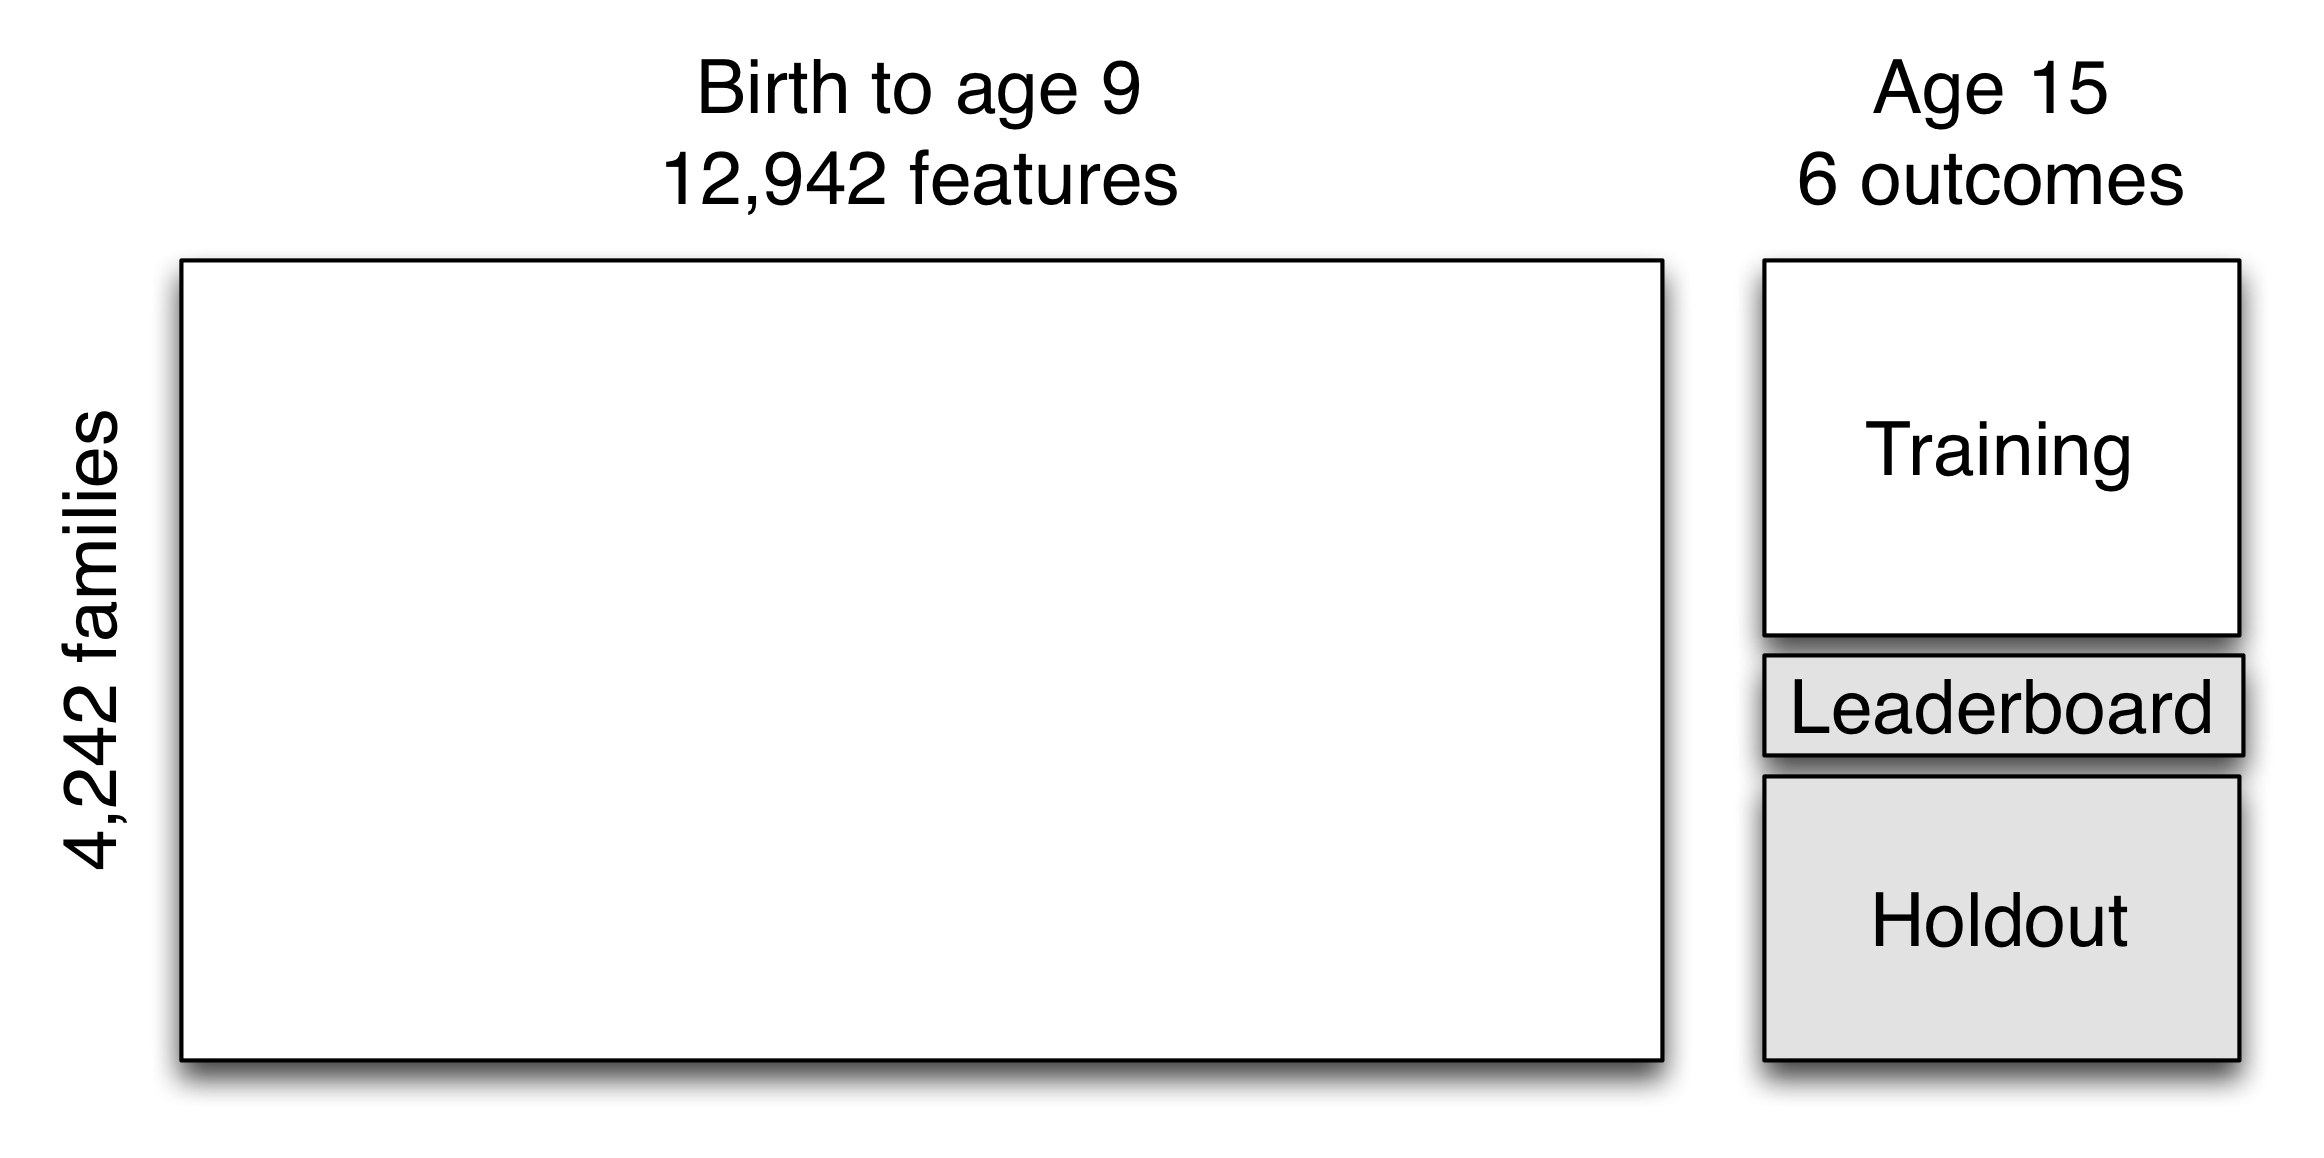
\includegraphics[height = .5\textheight]{figures/ffc_design_matrix_ml}};
\node<11> at (.5,.4) {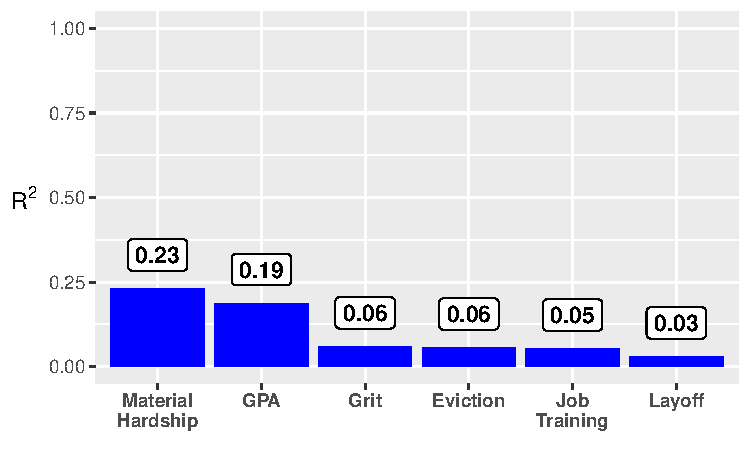
\includegraphics[height = .5\textheight]{figures/RSquared_all_ASA_01}};
\node<12>[draw, line width = 2pt, draw = blue, inner sep = 10pt, rounded corners, align = left, font = \large] at (.5,.4) {If you aim to\\\\--- \bblue{predict} an outcome well (our goal) or\\--- understand \bblue{all causes} of an outcome (harder)\\\\you are likely to be \bgreen{disappointed} with these data.\par};
\node[anchor = south west, font = \footnotesize,align=left] at (0,.03) {This slide is about the Fragile Families Challenge. Results are not yet published.\\You can read more \href{http://www.fragilefamilieschallenge.org}{\blue{here}} or watch a video overview \href{https://www.youtube.com/playlist?list=PLbavk6eDjgUSghfps3elbgD-uV8VAK4QH}{\blue{here}}.};
\end{tikzpicture}
\end{frame}



\begin{frame}
\begin{tikzpicture}[x = .5\textwidth, y = .5\textheight]
\node at (-1,-1) {};
\node at (1,1) {};
\node[anchor = west,font = \Large] at (-1, .8) {A \bblue{temptation}};
\node[anchor = west, align = left] at (-.9,.6) {Study \bgreen{all causes} of some outcome\\by throwing them all in a model.};
\node[font = \small, align = center, anchor = east] at (1, .6) {There are\\\bgreen{so many}\\variables!};
\draw[->, line width = 2pt, olive] (.65,.6) -- (.25, .6);
\node[anchor = west, font = \Large] at (-1, .2) {A \bblue{recommendation}};
\node[anchor = west, align = left] at (-.9,-.1) {Aim to answer a \bgreen{specific question}\\that can be stated\\without a regression model};
\node[anchor = west, align = left] at (-.9,-.4) {--- A specific question can be \bgreen{descriptive}};
\node[anchor = west, align = left] at (-.9,-.55) {--- A specific question can be \bgreen{causal}};
\only<1>{
\draw[rounded corners, line width = 3pt, gray] (-1,.45) rectangle (1, .9);
}
\only<2-3>{
\draw[rounded corners, line width = 3pt, gray] (-1,-.75) rectangle (1, .3);
}
\only<3>{
\draw[->, line width = 2pt, blue] (.8,-.4) -- (.45, -.4);
}
\end{tikzpicture}
\end{frame}

\begin{frame}
\centering
In the past 12 months, were you evicted from your home or apartment for not paying the rent or mortgage?\blfootnote{Paper published with Louis Donnelly \href{https://link.springer.com/article/10.1007/s13524-018-0735-y}{\blue{[link]}}} \vskip .5cm
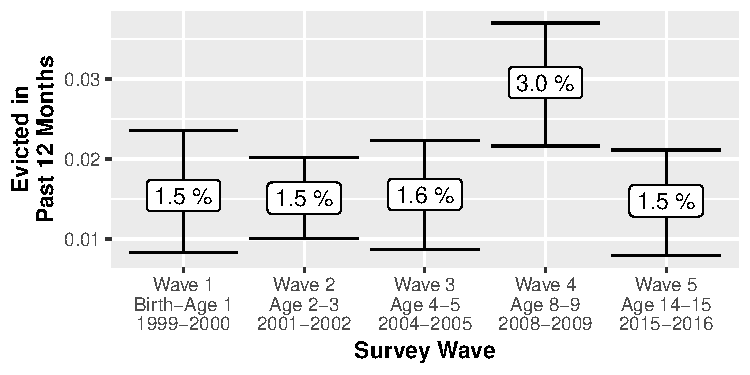
\includegraphics[width = \textwidth]{figures/evByWave_weightedOnly}
\end{frame}

\begin{frame}
\centering
\begin{tikzpicture}[x = .5\textwidth, y = .5\textheight]
\node at (-1,-1) {};
\node at (1,1) {};
\node[anchor = west] at (-1, .7) {Child ages covered by eviction reports};
\node at (0,0) {\includegraphics[width = \textwidth]{figures/evictionData_largeLabels}};
% Block out parts of figure I will highlight in other ways on slide
\draw[color = white, fill = white] (-1,0.2) rectangle (1,.4);
\draw[color = white, fill = white] (-1,0.02) rectangle (0,.11);
\draw[color = white, fill = white] (-1,-.08) rectangle (1,-.03);
\only<2-2>{
	\node (annual) at (0, .23) {12 months preceding each survey};
	\draw[line width = 1.5pt, blue, rounded corners] (-.9,.07) rectangle (.95,.32);
}
\only<3-3>{
	\node[align = center] at (0.5, .5) {Retrospective:\\Any eviction between\\ages 9 and 15};
	\draw[->, line width = 1.5pt, blue] (0.5, 0.3) -- (0.5, 0.07);
}
\only<4-4>{
	\node[align = center] at (-.38, .5) {Periods with no report};
	\draw[->, line width = 1.5pt, blue] (-.07, 0.45) -- (-.07, 0.15);
	\draw[->, line width = 1.5pt, blue] (-.43, 0.45) -- (-.43, 0.15);
	\draw[->, line width = 1.5pt, blue] (-.67, 0.45) -- (-.67, 0.15);
}
\only<5->{
\node at (0,.5) {\bblue{Goal:} Proportion evicted at any point};
\draw[|-|, blue, line width = 2pt] (-.85,.4) -- (.9, .4);
}
\only<6->{
\node[anchor = west] at (-.8, -.4) {Lower bound: \begin{Large}\bblue{7.9 \%}\end{Large} reported an eviction};
}
\onslide<7>{
\node[anchor = west] at (-.8, -.6) {Model-based: \begin{Large}\bblue{14.8 \%}\end{Large} evicted at some point};
\node[anchor = west, olive, font = \small] at (-.55, -.75) {Imputes over periods with no report};
\draw[->, line width = 1.5pt, olive] (-.65, -.65) to[out = 270, in = 180] (-.55, -.75);
}
\end{tikzpicture}
\end{frame}




\begin{frame}
\begin{tikzpicture}
\node at (0,0) {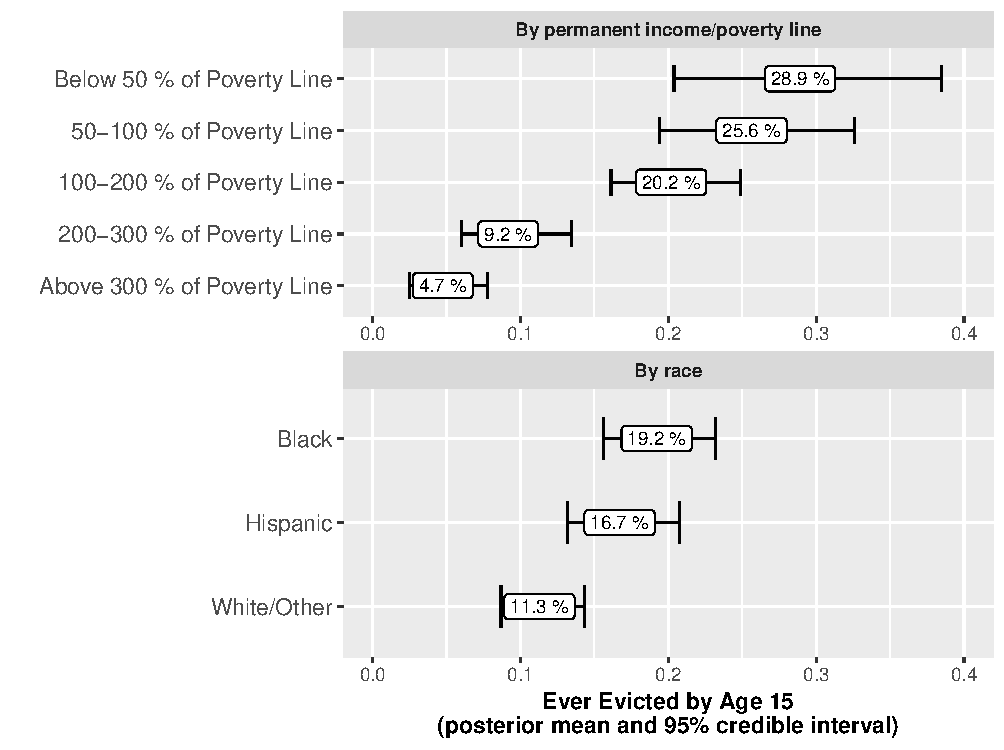
\includegraphics[width = \textwidth]{figures/RaceIncomeGroups_largeFont}};
\onslide<2>{
\node[fill = white, draw = blue, line width = 2.5pt, rounded corners, align=center] (oversample) at (4.2,-1.2) {Unmarried\\oversample\\aids\\ precision};
\draw[->, line width = 2pt, blue] (oversample) to[bend right] (4, 2.5);
\draw[->, line width = 2pt, blue] (3.13,-1) to[bend right] (2.5, -.7);
\draw[->, line width = 2pt, blue] (3.13,-1.7) to[bend left] (2.1, -1.7);
}
\end{tikzpicture}
\end{frame}

\begin{frame}
\begin{tikzpicture}[x = .5\textwidth, y = .5\textheight]
\node at (-1,-1) {};
\node at (1,1) {};
\node[anchor = west,font = \Large] at (-1, .8) {A \bblue{temptation}};
\node[anchor = west, align = left] at (-.9,.6) {Study \bgreen{all causes} of some outcome\\by throwing them all in a model.};
\node[font = \small, align = center, anchor = east] at (1, .6) {There are\\\bgreen{so many}\\variables!};
\draw[->, line width = 2pt, olive] (.65,.6) -- (.25, .6);
\node[anchor = west, font = \Large] at (-1, .2) {A \bblue{recommendation}};
\node[anchor = west, align = left] at (-.9,-.1) {Aim to answer a \bgreen{specific question}\\that can be stated\\without a regression model};
\node[anchor = west, align = left] at (-.9,-.4) {--- A specific question can be \bgreen{descriptive}};
\node[anchor = west, align = left] at (-.9,-.55) {--- A specific question can be \bgreen{causal}};
\draw[rounded corners, line width = 3pt, gray] (-1,-.75) rectangle (1, .3);
\only<1>{
\draw[->, line width = 2pt, blue] (.8,-.4) -- (.45, -.4);
}
\only<2>{
\draw[->, line width = 2pt, blue] (.8,-.55) -- (.45, -.55);
}
\end{tikzpicture}
\end{frame}

\begin{frame}
\centering\large
Does \bblue{public housing} protect\\low-income families from \bblue{eviction}?\blfootnote{Draft with Sarah Gold, Louis Donnelly,\\Jeanne Brooks-Gunn, and Sara McLanahan \href{http://paa2019.populationassociation.org/uploads/192630}{\blue{[link]}}} \vskip .6cm
\begin{tikzpicture}[x = .8\textwidth]
\node at (-.13, -2.5) {};
\node at (1.125, 0) {};
\onslide<2-4>{
\draw[|-, thick] (0,0) -- (9/15,0);
\node[anchor = south, align=center, font = \footnotesize] at (0,.1) {Age 0};
}
\onslide<5->{
\draw[|-, thick, gray] (0,0) -- (9/15,0);
\node[anchor = south, align=center, font = \footnotesize, gray] at (0,.1) {Age 0};
}
\onslide<2->{
\draw[|-|, thick] (9/15,0) -- (1,0);
\node[anchor = south, align=center, font = \footnotesize] at (9/15,.1) {Age 9};
\node[anchor = south, align=center, font = \footnotesize] at (1,.1) {Age 15};
}
\only<3-4>{
\node[anchor = north,align=center, font = \footnotesize] at (0,-.1) {Born 1998--2000\\large U.S. city};
}
\only<4>{
\draw[|-|, thick] (0,-1.3) -- (9/15,-1.3);
\node[anchor = north,align=center, font = \footnotesize, fill = white] at (4.5/15,-1) {Family income\\ever below 200 \%\\federal poverty line};
% for family of 4 (2 adults and 2 kids) that would be 51k in 2018
}
\only<5->{
\node[anchor = north,align=center, font = \footnotesize, gray] at (0,-.1) {Born 1998--2000\\large U.S. city};
\draw[|-|, thick, gray] (0,-1.3) -- (9/15,-1.3);
\node[anchor = north,align=center, font = \footnotesize, fill = white, text = gray] at (4.5/15,-1) {Family income\\ever below 200 \%\\federal poverty line};
}
\onslide<6->{
\node[anchor = north,align=center, font = \footnotesize] at (9/15,-.1) {Resides in\\\bblue{public housing}};
}
\onslide<7->{
\draw[|-|, thick] (9/15,-1.3) -- (15/15,-1.3);
\node[anchor = north,align=center, font = \footnotesize, fill = white] at (12/15,-1) {Ever \bblue{evicted}?};
}
\end{tikzpicture} %\vskip .3cm
%For those residing in public housing,\\how much does assistance reduce $\P(\text{Eviction})$?
\end{frame}

\begin{frame}{Effect of \bblue{public housing} on \bblue{eviction}}
\centering
\begin{tikzpicture}
\node<1> at (0,0) {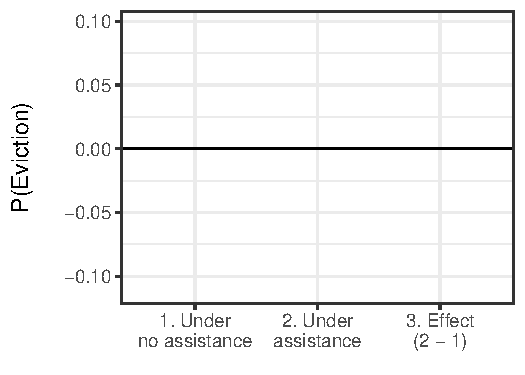
\includegraphics[height = .8\textheight]{figures/effect_public_evicted_0_}};
\node<2> at (0,0) {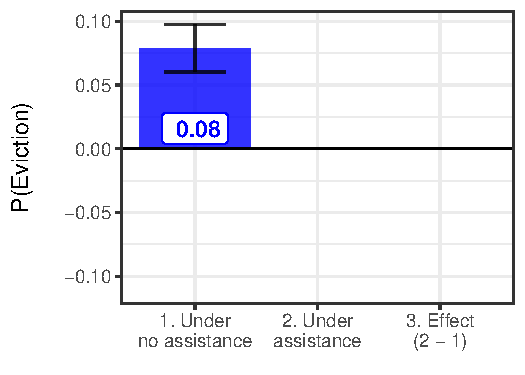
\includegraphics[height = .8\textheight]{figures/effect_public_evicted_1_}};
\node<3> at (0,0) {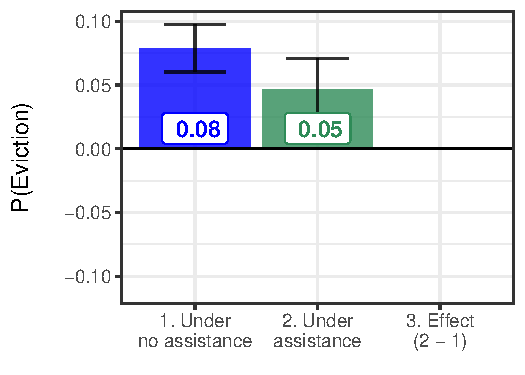
\includegraphics[height = .8\textheight]{figures/effect_public_evicted_2_}};
\node<4> at (0,0) {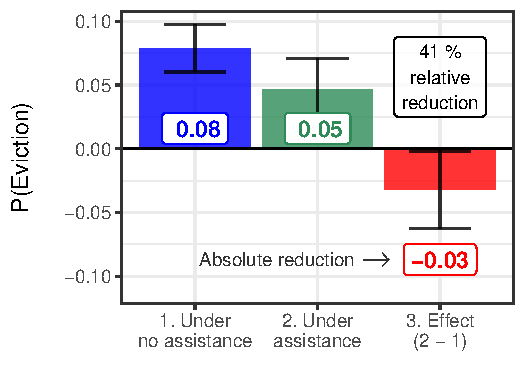
\includegraphics[height = .8\textheight]{figures/effect_public_evicted_3_}};
\end{tikzpicture}
\end{frame}

\begin{frame}
\begin{tikzpicture}[x = .5\textwidth, y = .5\textheight]
\node at (-1,-1) {};
\node at (1,1) {};
\node[anchor = west,font = \Large] at (-1, .8) {A \bblue{temptation}};
\node[anchor = west, align = left] at (-.9,.6) {Study \bgreen{all causes} of some outcome\\by throwing them all in a model.};
\node[font = \small, align = center, anchor = east] at (1, .6) {There are\\\bgreen{so many}\\variables!};
\draw[->, line width = 2pt, olive] (.65,.6) -- (.25, .6);
\node[anchor = west, font = \Large] at (-1, .2) {A \bblue{recommendation}};
\node[anchor = west, align = left] at (-.9,-.1) {Aim to answer a \bgreen{specific question}\\that can be stated\\without a regression model};
\node[anchor = west, align = left] at (-.9,-.4) {--- A specific question can be \bgreen{descriptive}};
\node[anchor = west, align = left] at (-.9,-.55) {--- A specific question can be \bgreen{causal}};
\draw[rounded corners, line width = 3pt, gray] (-1,-.75) rectangle (1, .3);
\end{tikzpicture}
\end{frame}

\begin{frame}{Cautionary notes}
\begin{tikzpicture}[x = \textwidth, y = \textheight]
\node at (0,0) {};
\node at (1,1) {};
\node[anchor = west] at (0,.8) {\bblue{Target population}: Describe carefully};
\node[anchor = north west] at (.05,.75) {--- \bred{Not} Nationally representative};
\node[anchor = north west] at (.05,.7) {--- \bred{Not} Residents of cities};
\node[anchor = north west, align = left] at (.05,.65) {--- \bgreen{Yes} Probability sample of births in U.S. cities\\\hspace{34pt} with populations over 200,000 in 1998--2000};
\onslide<2->{
\node[anchor = west] at (0,.45) {\bblue{Oversample}: Describe carefully};
\node[anchor = north west] at (.05,.4) {--- \bred{Not} Oversample of disadvantaged families};
\node[anchor = north west, align = left] at (.05,.35) {--- \bgreen{Yes} Oversample (3:1) of nonmarital births};
}
\onslide<3->{
\node[font = \footnotesize, anchor = east, align = center] at (1,.2) {Tendency toward disadvantage\\is a \bblue{consequence} of\\this.};
\draw[->, thick, olive] (.95, .25) to[bend right] (.8, .375);
\draw[->, thick, olive] (.75, .15) to[out = 180, in = 290] (.27, .28);
}
\end{tikzpicture}
\end{frame}

\begin{frame}{Cautionary notes}

\vskip .2cm
\bblue{Weights} are highly unequal.\\
\begin{center}
\begin{tikzpicture}
\onslide<2->{
\node[font = \bf] at (0, 3) {National mother weights at birth};
\node[font = \Large, align = center] at (0.5, -3.2) {Proportion\\of \bblue{sample}};
\node[font = \Large, align = center] at (-3.8, .2) {Proportion\\of \bblue{weight}};
}
\node<2> at (0,0) {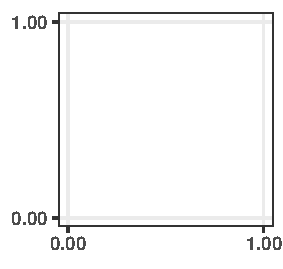
\includegraphics[width = .5\textwidth]{figures/weight_issue_0}};
\node<3> at (0,0) {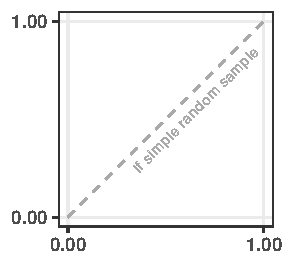
\includegraphics[width = .5\textwidth]{figures/weight_issue_1}};
\node<4> at (0,0) {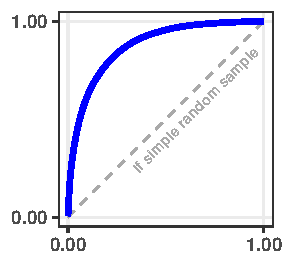
\includegraphics[width = .5\textwidth]{figures/weight_issue_2}};
\node<5-> at (0,0) {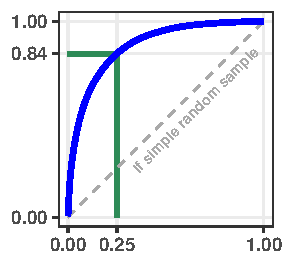
\includegraphics[width = .5\textwidth]{figures/weight_issue_3}};
\onslide<6>{
\node[align=center, font = \large] at (-5,-2) {\bgreen{84 \%} of weight rests\\on \bgreen{25 \%} of sample};
\draw[->, line width = 2pt, color = olive] (-6.5, -1.5) to[out = 90, in = 180] (-2.7, 1.5);
\draw[->, line width = 2pt, color = olive] (-5.7, -2.5) to[out = 270, in = 210] (-1, -2.5);
}
%\node[align = left, font = \footnotesize] at (-5, .5) {Weights are not bad.\\They are just high-variance.\\This is a consequence of the heavy oversample\\that enables precise estimates for non-marital births.\\\\\bblue{Advice:} Think carefully about whether to weight.\\Weighted and unweighted samples are very different.};
\end{tikzpicture}
\end{center}
\end{frame}

\begin{frame}{Cautionary notes}
\begin{center}
\scalebox{.4}{
\begin{tikzpicture}\
\node[font = \bf] at (0, 3) {National mother weights at birth};
\node[font = \Large, align = center] at (0.5, -3.2) {Proportion\\of \bblue{sample}};
\node[font = \Large, align = center] at (-3.8, .2) {Proportion\\of \bblue{weight}};\
\node at (0,0) {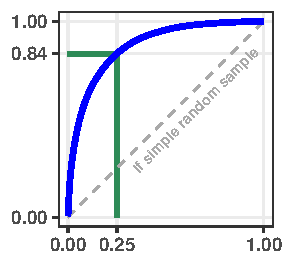
\includegraphics[width = .5\textwidth]{figures/weight_issue_3}};
\node[align=center, font = \large] at (-5,-2) {\bgreen{84\%} of weight rests\\on \bgreen{25 \%} of sample};
\draw[->, line width = 2pt, color = olive] (-6.5, -1.5) to[out = 90, in = 180] (-2.7, 1.5);
\draw[->, line width = 2pt, color = olive] (-5.7, -2.5) to[out = 270, in = 210] (-1, -2.5);
%\node[align = left, font = \footnotesize] at (-5, .5) {Weights are not bad.\\They are just high-variance.\\This is a consequence of the heavy oversample\\that enables precise estimates for non-marital births.\\\\\bblue{Advice:} Think carefully about whether to weight.\\Weighted and unweighted samples are very different.};
\end{tikzpicture}
}
\end{center}
Weights are not bad.\vskip .2cm
They are just high-variance.\vskip .2cm
This is a consequence of the oversample\\that enables precise estimates for non-marital births.\vskip .2cm
\bblue{Advice:} Think carefully about whether to weight.\\
\hspace{44pt}Weighted and unweighted samples are very different.

\end{frame}

%\begin{frame}{Cautionary notes}
%Think a bit about \bblue{statistical power}. \vskip .5in
%Sample is large (4,898) but not huge. Start with a crosstab.
%\end{frame}

\begin{frame}{Comparison to other datasets}

\bblue{Gaps} between surveys: Not annual
\begin{center}
\includegraphics[width = \textwidth, trim = 0in .06in 0in .23in, clip]{figures/evictionData_largeLabels}
\end{center} \vskip .3cm
\bblue{Target population} is specific. \quad \begin{footnotesize}(but so is NLSY-CYA and PSID-CDS)\end{footnotesize}\vskip .5cm
Many \bblue{likert-type} scales influenced by psychology
\end{frame}



\begin{frame}{Opportunities}

There are lots of variables no one is studying.\\
\bblue{Pick a variable and run with it!} \vskip .1in
\begin{tikzpicture}[x = .5\textwidth, y = .5\textheight]
%%%%%%%%%%%%%%%%%%%%%%
\onslide<2->{
\node[anchor = west] at (-1, .2) {A \bblue{recommendation}};
\node[anchor = west, align = left, font = \small] at (-1,-.1) {Aim to answer a \bgreen{specific question}\\that can be stated\\without a regression model};
\node[anchor = west, align = left, font = \small] at (-1,-.4) {--- A specific question can be \bgreen{descriptive}};
\node[anchor = west, align = left, font = \small] at (-1,-.55) {--- A specific question can be \bgreen{causal}};
%\draw[line width = 3pt, gray] (.2, .3) -- (.2,-.75);
\draw[rounded corners, line width = 3pt, gray] (-1,-.75) rectangle (.2, .3);
}
%%%%%%%%%%%%%%%%%%%%%%
\onslide<3->{
\node at (.6, .4) {Words of \bblue{caution}};
\draw[thick] (.3, .33) -- (.9, .33);
}
\onslide<4->{
\node[font = \footnotesize, align = center, rotate = 20] at (.6, .15) {Target population:\\births in cities};
\node[font = \footnotesize, rotate = -15] at (.6, -.15) {Nonmarital oversample};
\node[font = \footnotesize, rotate = 10] at (.6, -.4) {Unequal weights};
};
\onslide<5->{
\node[align=center] at (.6, -.7) {For the right question,\\these are \bblue{advantages}};
}
\end{tikzpicture}
\end{frame}

\begin{frame}
\begin{Large}\textbf{Slides}: \blue{\href{https://github.com/ilundberg/slides}{github.com/ilundberg/slides}}\end{Large} \vskip .5cm
\textbf{References} \vskip .1cm
\begin{footnotesize}
Lundberg, Ian, and Louis Donnelly. 2019. \href{https://link.springer.com/article/10.1007/s13524-018-0735-y}{\blue{``A research note on the prevalence of housing eviction among children born in U.S. cities.''}} \emph{Demography} 56(1):391-404. [\href{https://scholar.princeton.edu/sites/default/files/ilundberg/files/lundbergdonnelly2019_accepted.pdf}{\blue{accepted manuscript}}][\href{https://doi.org/10.7910/DVN/BVWFG1}{\blue{replication package}}]. \vskip .3cm
Lundberg, Ian, Sarah L. Gold, Louis Donnelly, Jeanne Brooks-Gunn, and Sara S. McLanahan. \href{http://paa2019.populationassociation.org/uploads/192630}{\blue{``Government assistance protects low-income families from eviction and rent non-payment.''}} To be presented at the 2019 Annual Meeting of the Population Association of America.
\vskip .3cm
Salganik, Matthew J., Ian Lundberg, Alex Kindel, Sara S. McLanahan, and over 100 additional authors. ``Measuring the predictability of life outcomes with a scientific mass collaboration.'' Manuscript in progress.\\Read more \href{http://www.fragilefamilieschallenge.org}{\blue{here}} or watch a video overview \href{https://www.youtube.com/playlist?list=PLbavk6eDjgUSghfps3elbgD-uV8VAK4QH}{\blue{here}}.
\end{footnotesize}\vskip .4cm
\begin{minipage}{\textwidth}
\tiny
Research reported in this presentation was supported by The Eunice Kennedy Shriver National Institute of Child Health \& Human Development of the National Institutes of Health under Award Number P2CHD047879, R01HD36916, R01HD39135, and R01HD40421, as well as a consortium of private foundations. For the Fragile Families Challenge, we are especially grateful to the Russell Sage Foundation. The content is solely the responsibility of the authors and does not necessarily represent the official views of the National Institutes of Health.
\end{minipage}
\end{frame}



\end{document}